%********************************************************************
% Appendix
%*******************************************************
% If problems with the headers: get headings in appendix etc. right
%\markboth{\spacedlowsmallcaps{Appendix}}{\spacedlowsmallcaps{Appendix}}
\chapter{Appendix}

\section{Traktor zu Pixel Verhältnis} \label{apx:res}
Hier wird das Pixel zu Meter Verhältnis untersucht, also auf wie vielen Pixeln des Kamerabildes ein realer Meter abgebildet wird.
Dies ist relevant wenn es darum geht, den Traktor zu erkennen.

\bigskip
Zur Veranschaulichung dient Abbildung \ref{fig:apx:px_m}, welche das Sichtfeld aus der Vogelperspektive zeigt.
Dabei ist folgendes gegeben:
\begin{itemize}
    \item Die Montagehöhe der Kamera $s_1$;
    \item Die Sichtweite der Kamera $s_2$ (in unserem Anwendungsfall 300m);
    \item Die daraus resultierende Sichtstrecke bis zur Grenze: $A = \sqrt{s_l^2 + s_w^2}$;
    \item Sichtfeld $\alpha$, welches dem horizontalem Öffnungswinkel der Kamera entspricht.
\end{itemize}

\begin{figure}[!hbt]
    \center
    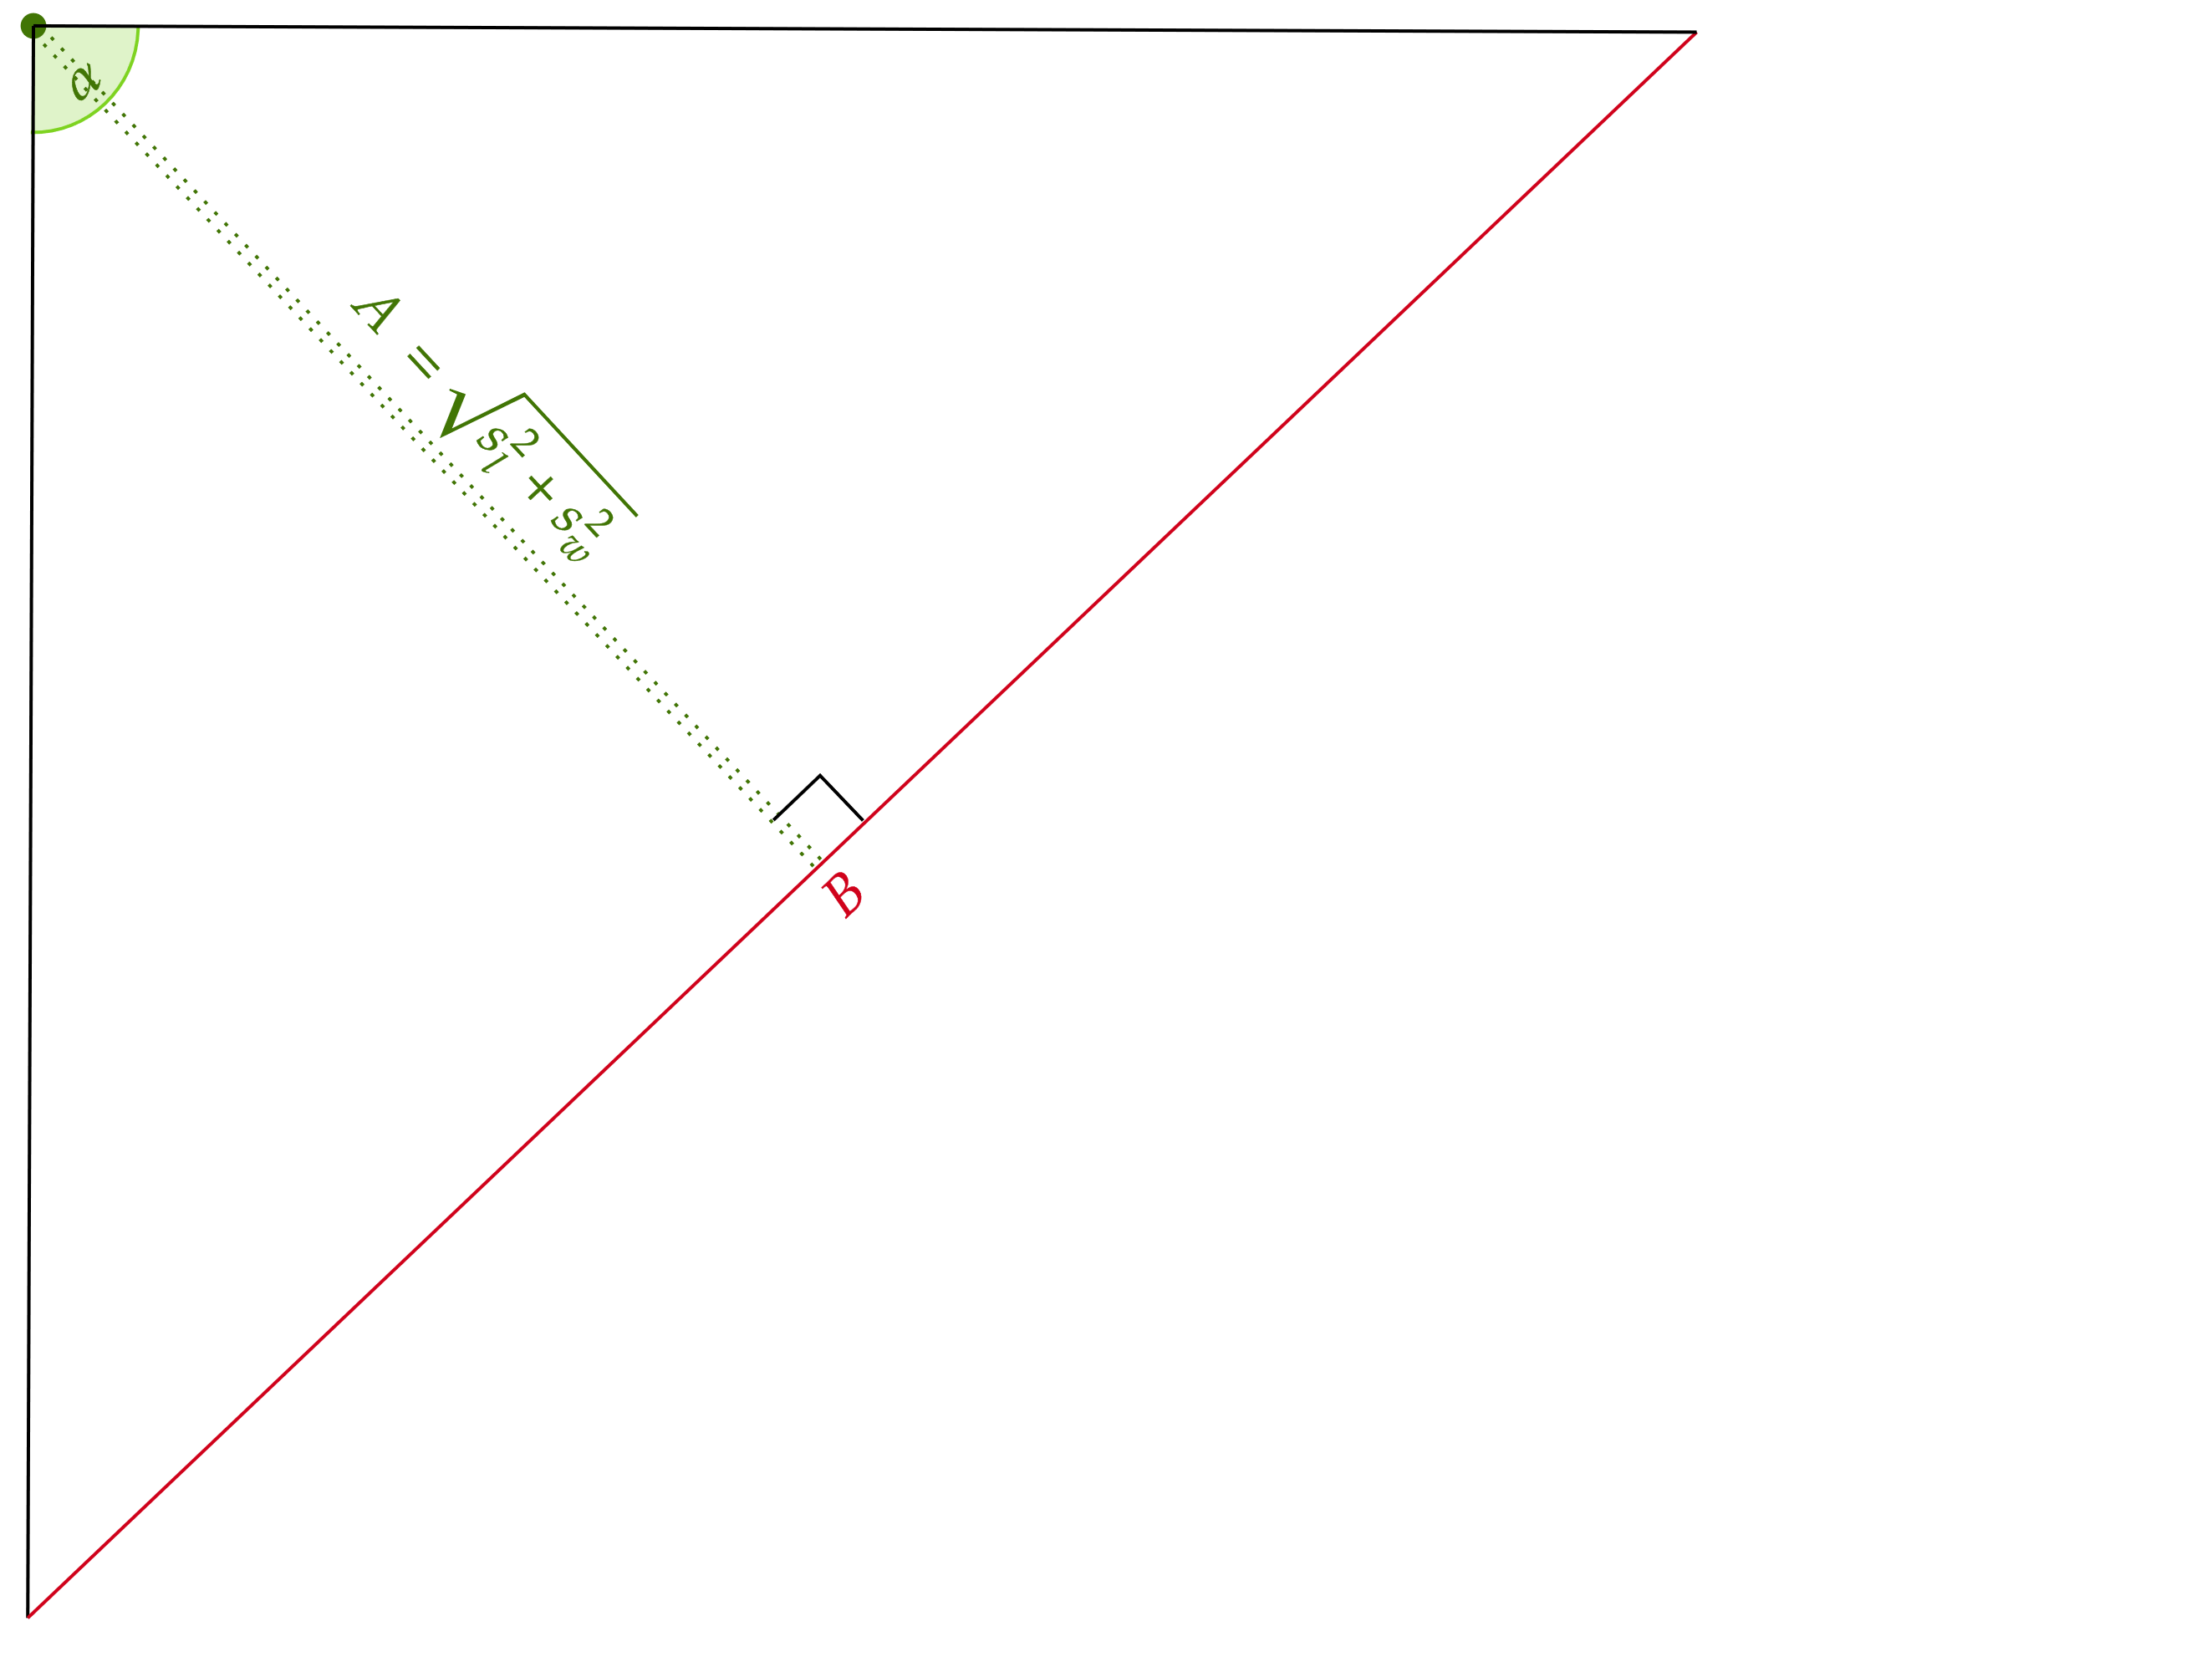
\includegraphics[width=0.95\textwidth]{figures/appendix/camera_bird}
    \caption{Skizze zur Berechnung des Pixel zu Meter Verhältnisses}
    \label{fig:apx:px_m}
\end{figure}

Zur Berechnung der Breite $B$ gilt allgemein Gleichung \ref{math:apx:b}.
\begin{flalign}
    \label{math:apx:b}
    \tan(\alpha/2) &= \frac{B/2}{A} \\
        B &= 2 \cdot \tan(\alpha/2) \cdot A
\end{flalign}

\bigskip
Ist die Sichtbreite der Kamera bestimmt, kann die nötige Auflösung der Kamera berechnet werden. 
Dazu sei weiter bekannt:
\begin{itemize}
    \item $o$, die Mindestgröße, die der Traktor im Bild einnehmen muss;
    \item $T$, die Traktorgröße in Echt;
    \item $B$, eben bestimmte Breite.
\end{itemize}

Zum Bestimmen der Auflösung wird berechnet, wie oft ein Traktor in das Sichtfeld hinein passt.
Die Anzahl der Traktoren wird dann mit der Mindestgröße $o$ multipliziert.
Das Produkt gibt die entsprechende horizontale Auflösung der Kamera an.

\begin{flalign}
    \label{math:apx:res}
    \text{Auflösung} &= o \cdot \frac{B}{T}
\end{flalign}


\section{BGS IoU Vergleich} \label{apx:bgs_iou}
In \autoref{fig:apx:bgs_iou_1} und \autoref{fig:apx:bgs_iou_2} sind die \acp{IoU} zu sehen.
Dabei fällt auf, dass bei Nacht die markierten und gefundenen Boxen sich stark unterscheiden.
Der \ac{BGS} findet vor allem das Licht bzw. den Lichtkegel.
Das führt zu geringen \acp{IoU}.

\begin{figure}[H]
    \centering
    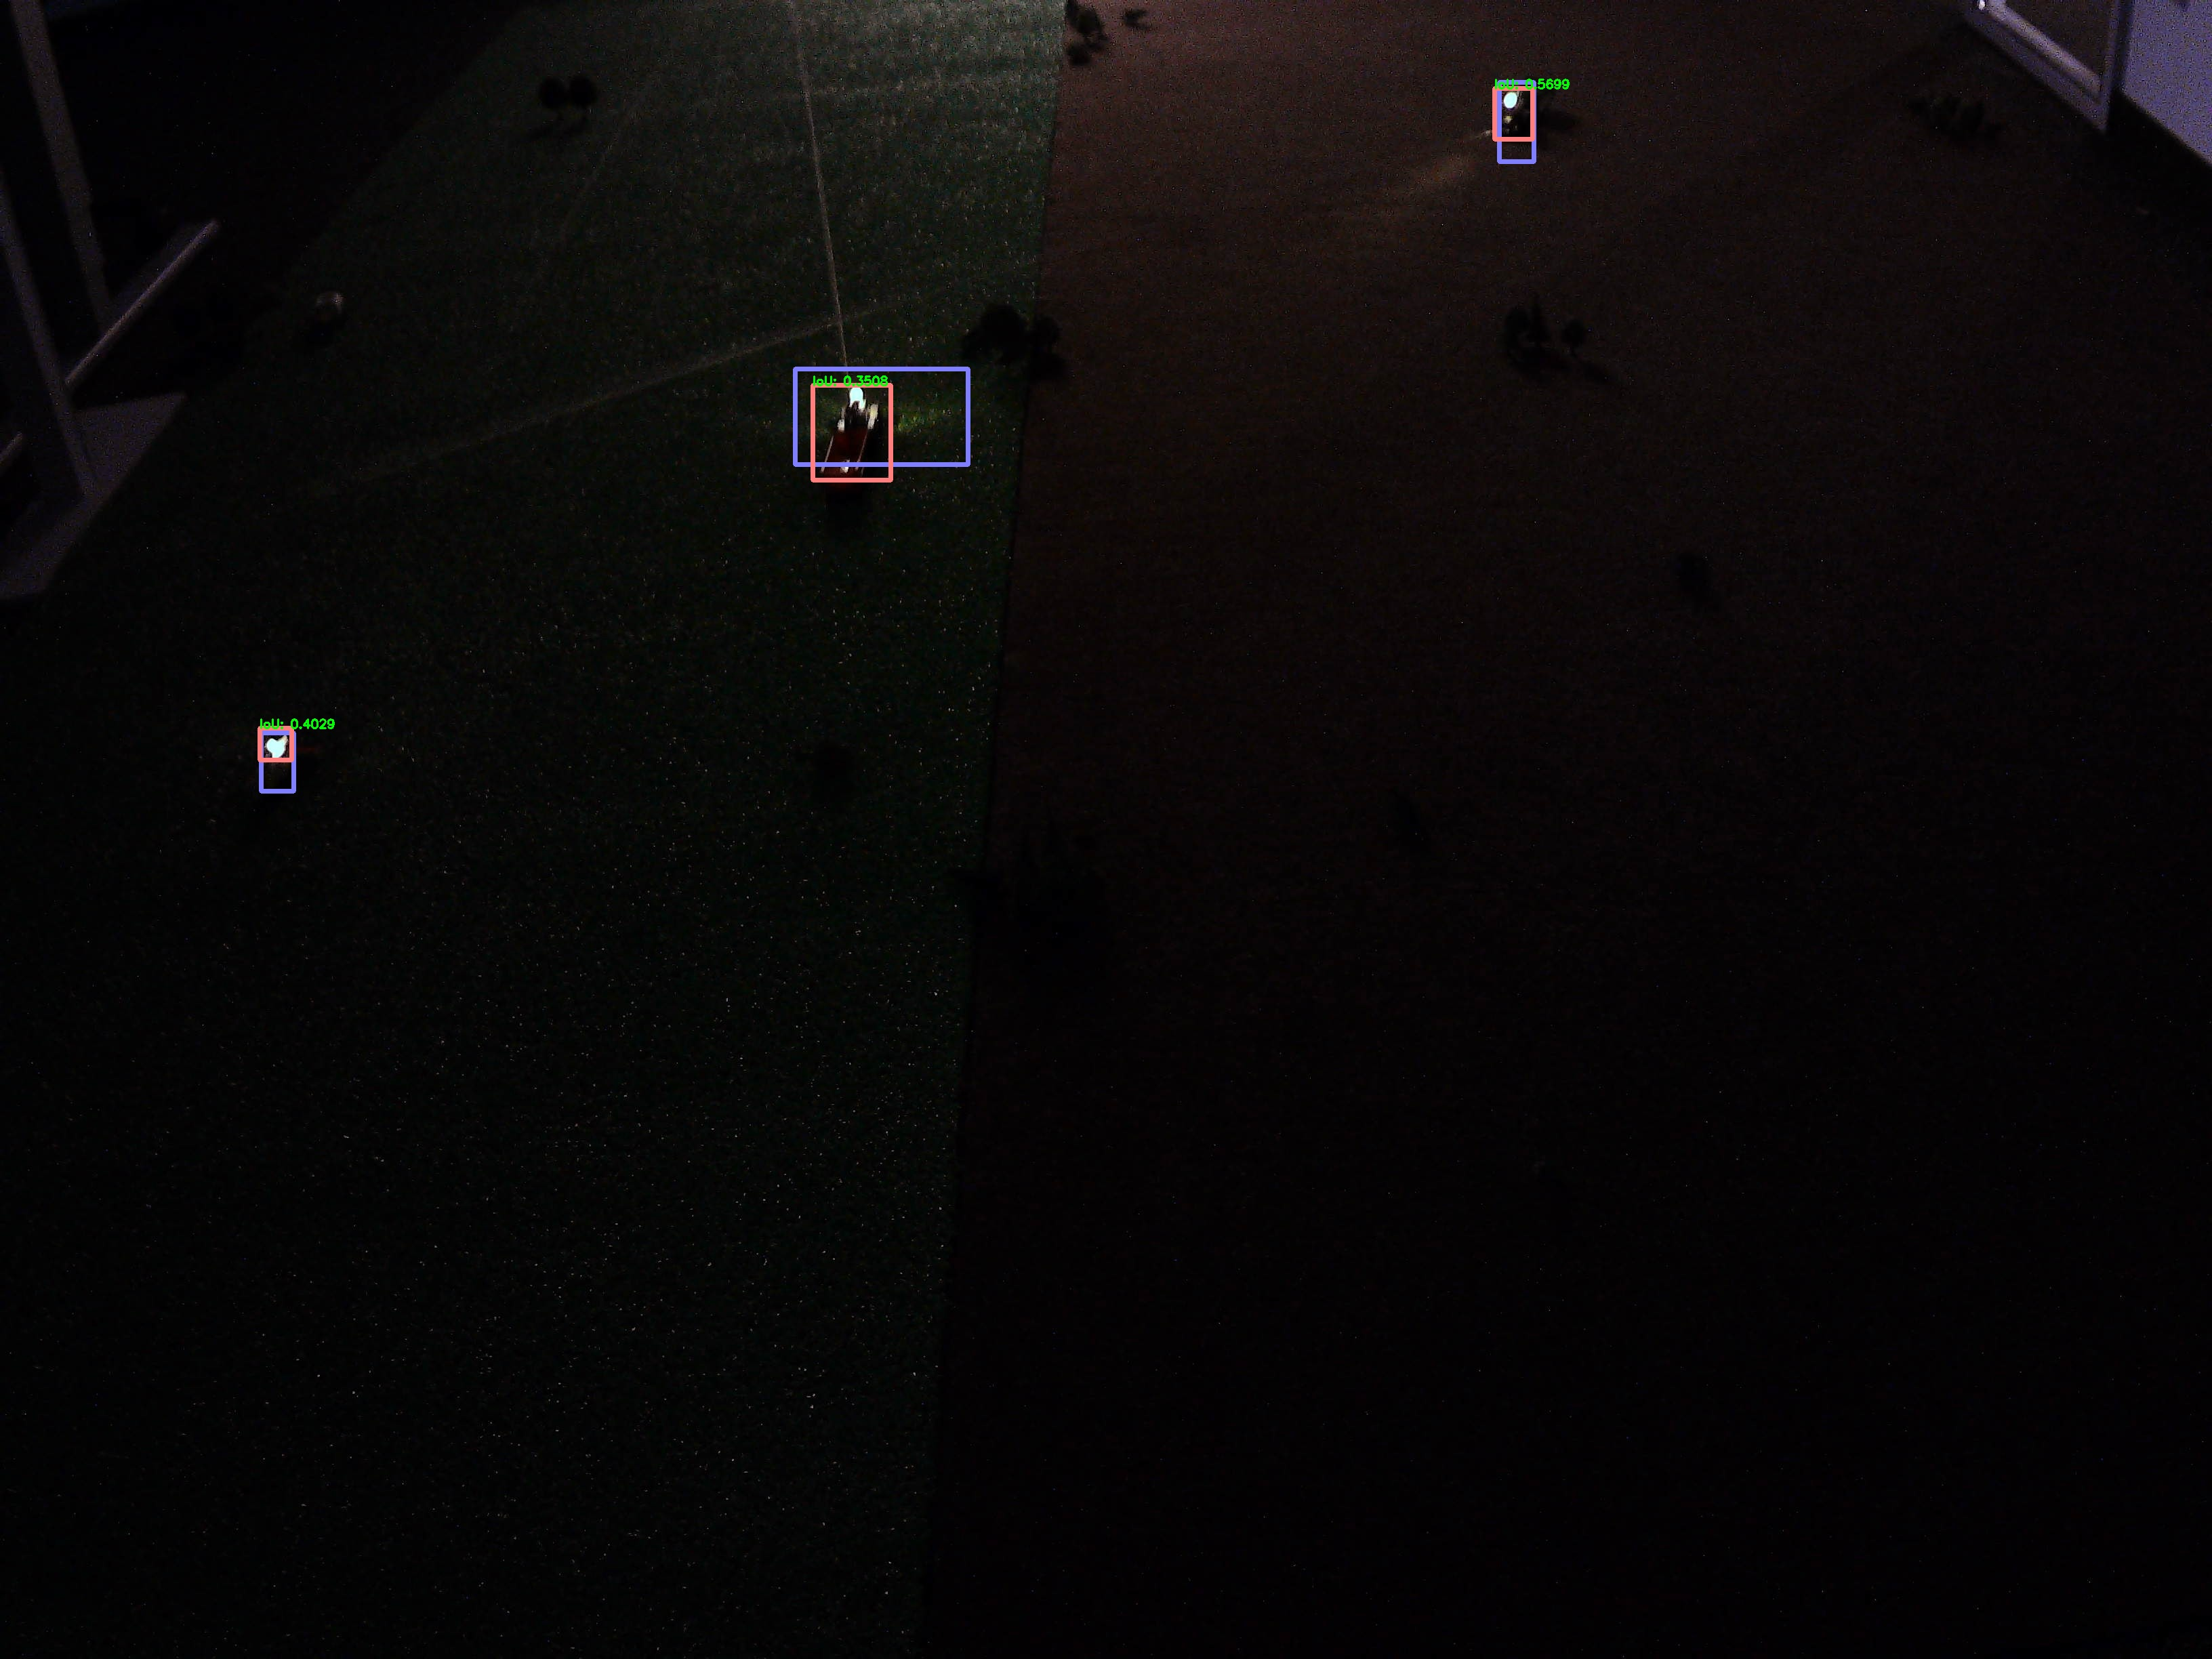
\includegraphics[width=0.95\textwidth]{figures/appendix/bgs_iou_1}
    \caption[IoU bei Nacht]{IoU bei Nacht: Rot kennzeichnet die händisch markierte Bounding Box und Blau die vom \ac{BGS} gefundene.}
    \label{fig:apx:bgs_iou_1}
\end{figure}
\begin{figure}[H]
    \centering
    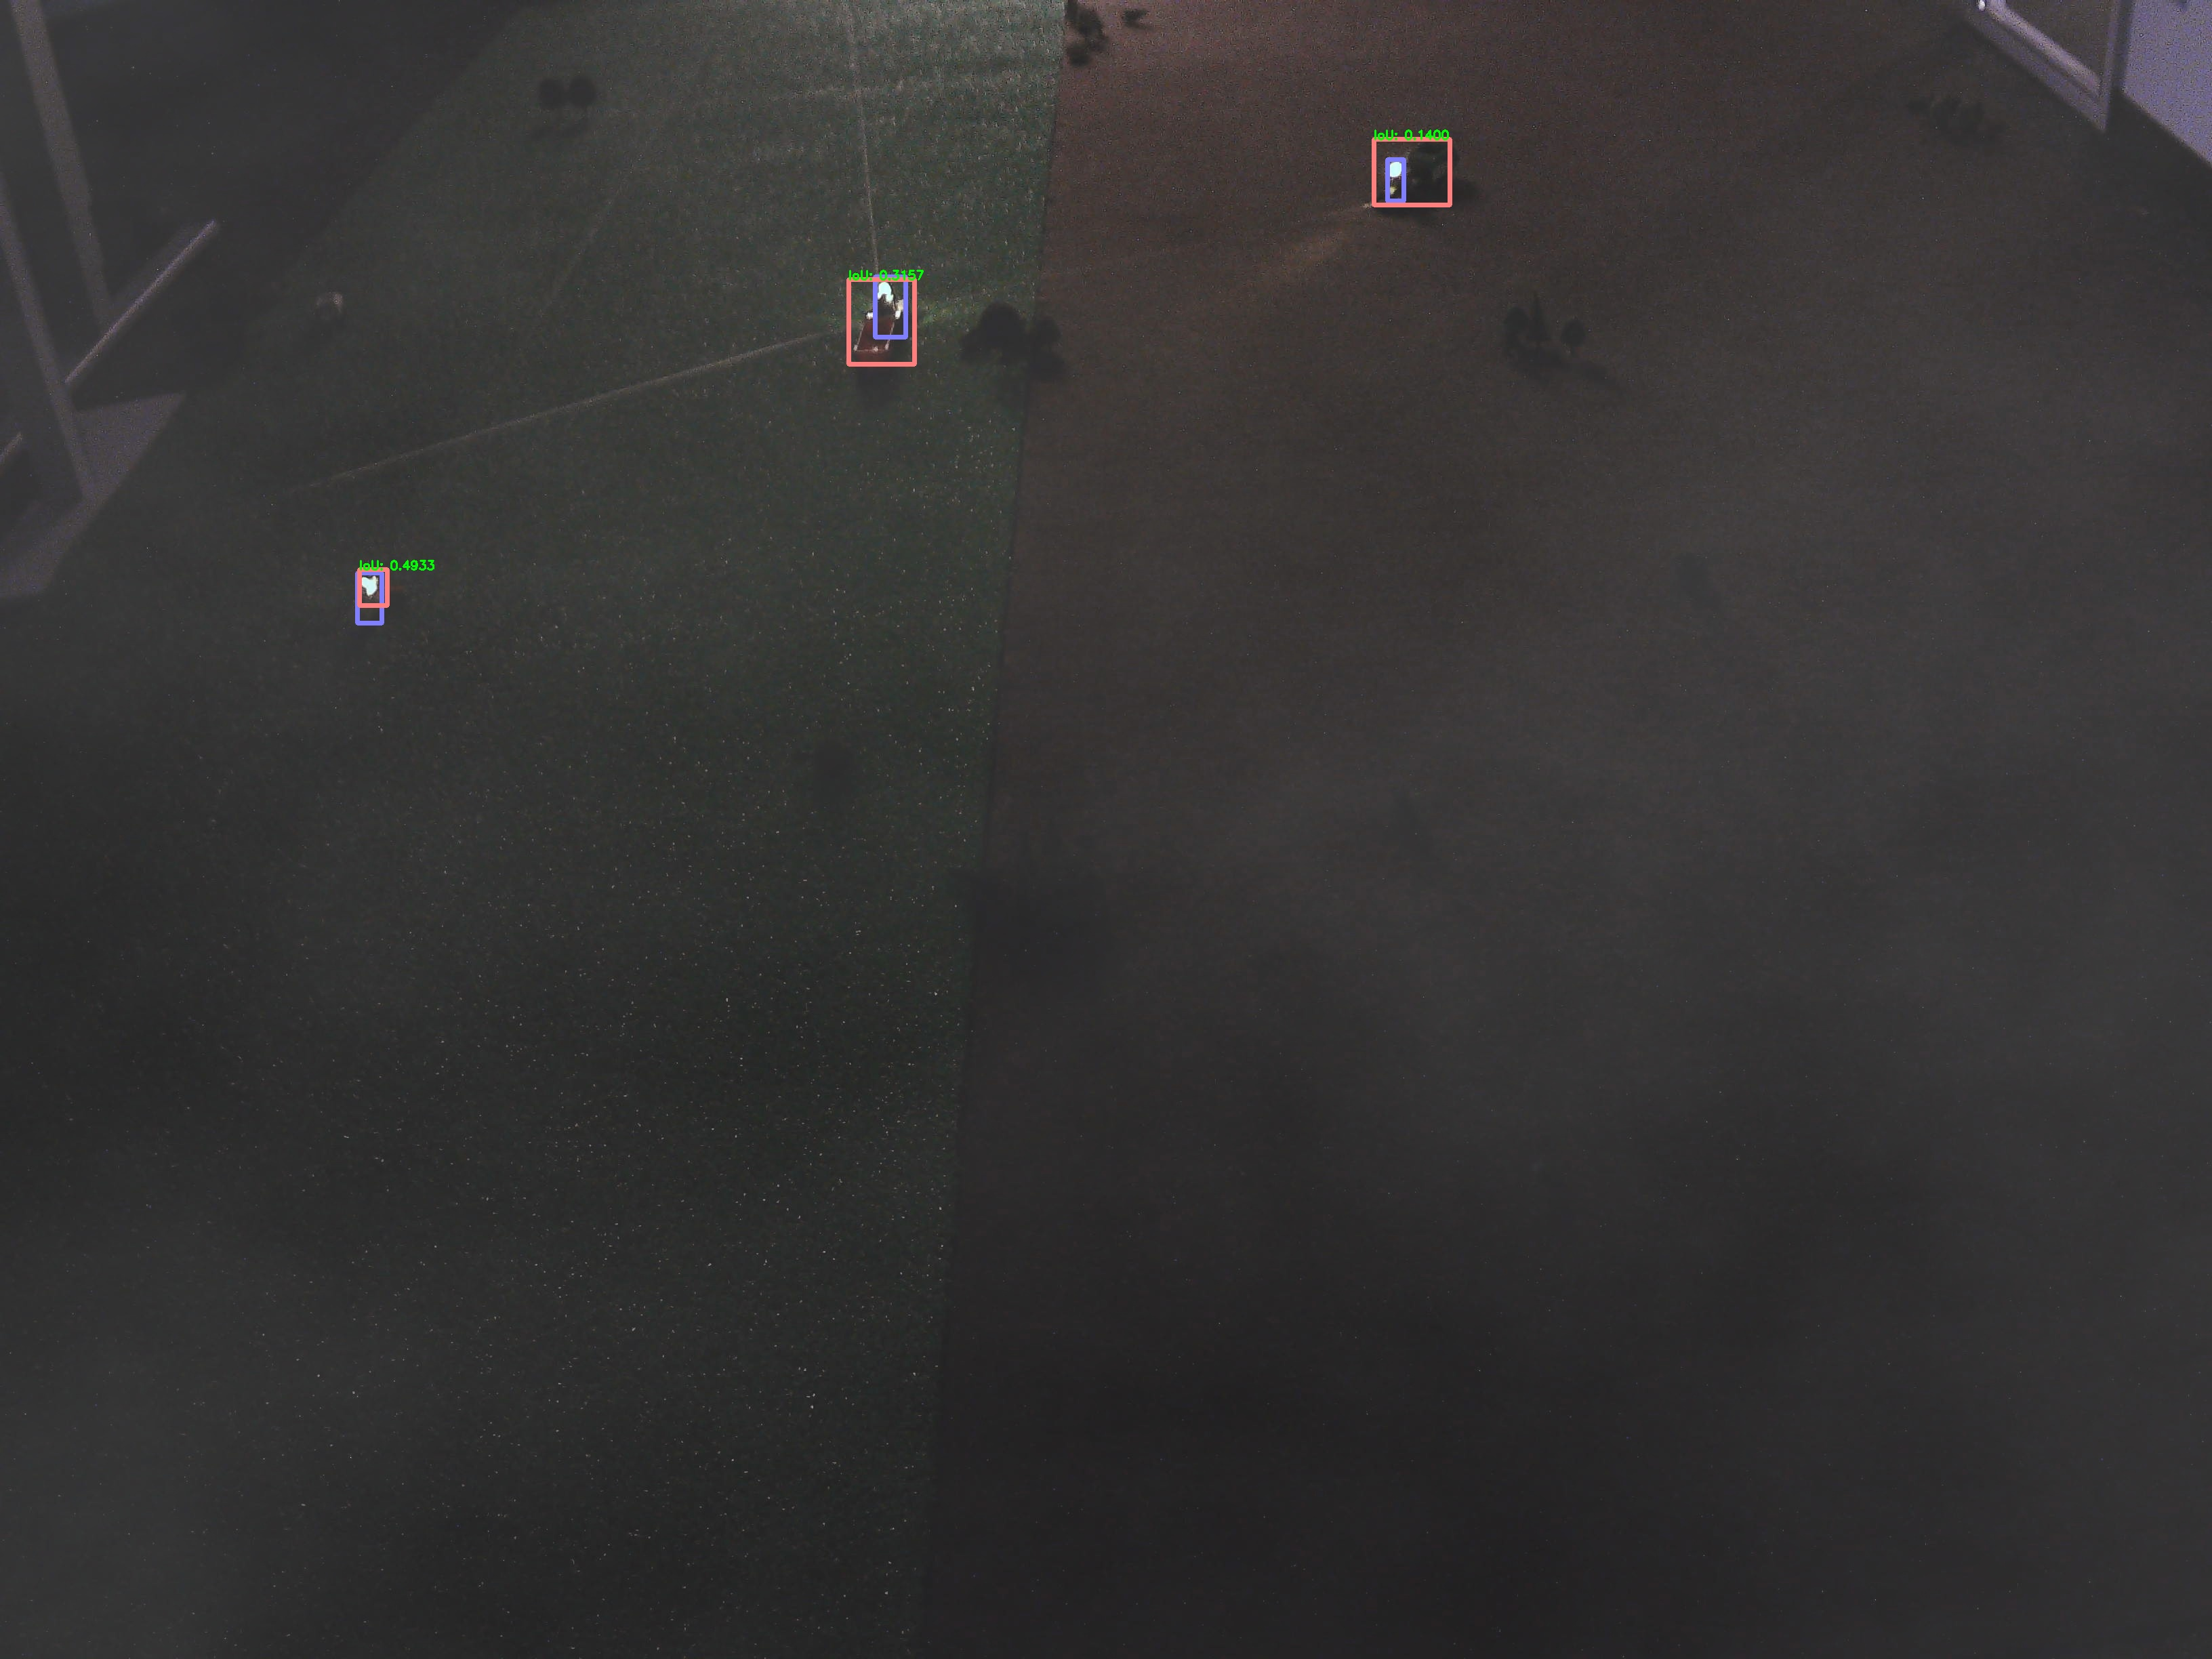
\includegraphics[width=0.95\textwidth]{figures/appendix/bgs_iou_2}
    \caption[IoU bei Nacht und Nebel]{IoU bei Nacht und Nebel: Rot kennzeichnet die händisch markierte Bounding Box und Blau die vom \ac{BGS} gefundene.}
    \label{fig:apx:bgs_iou_2}
\end{figure}

\section{Lernrate Range Test} \label{apx:lr_rangetest}
\subsection*{EFN-N5}
\begin{figure}[H]
    \centering
    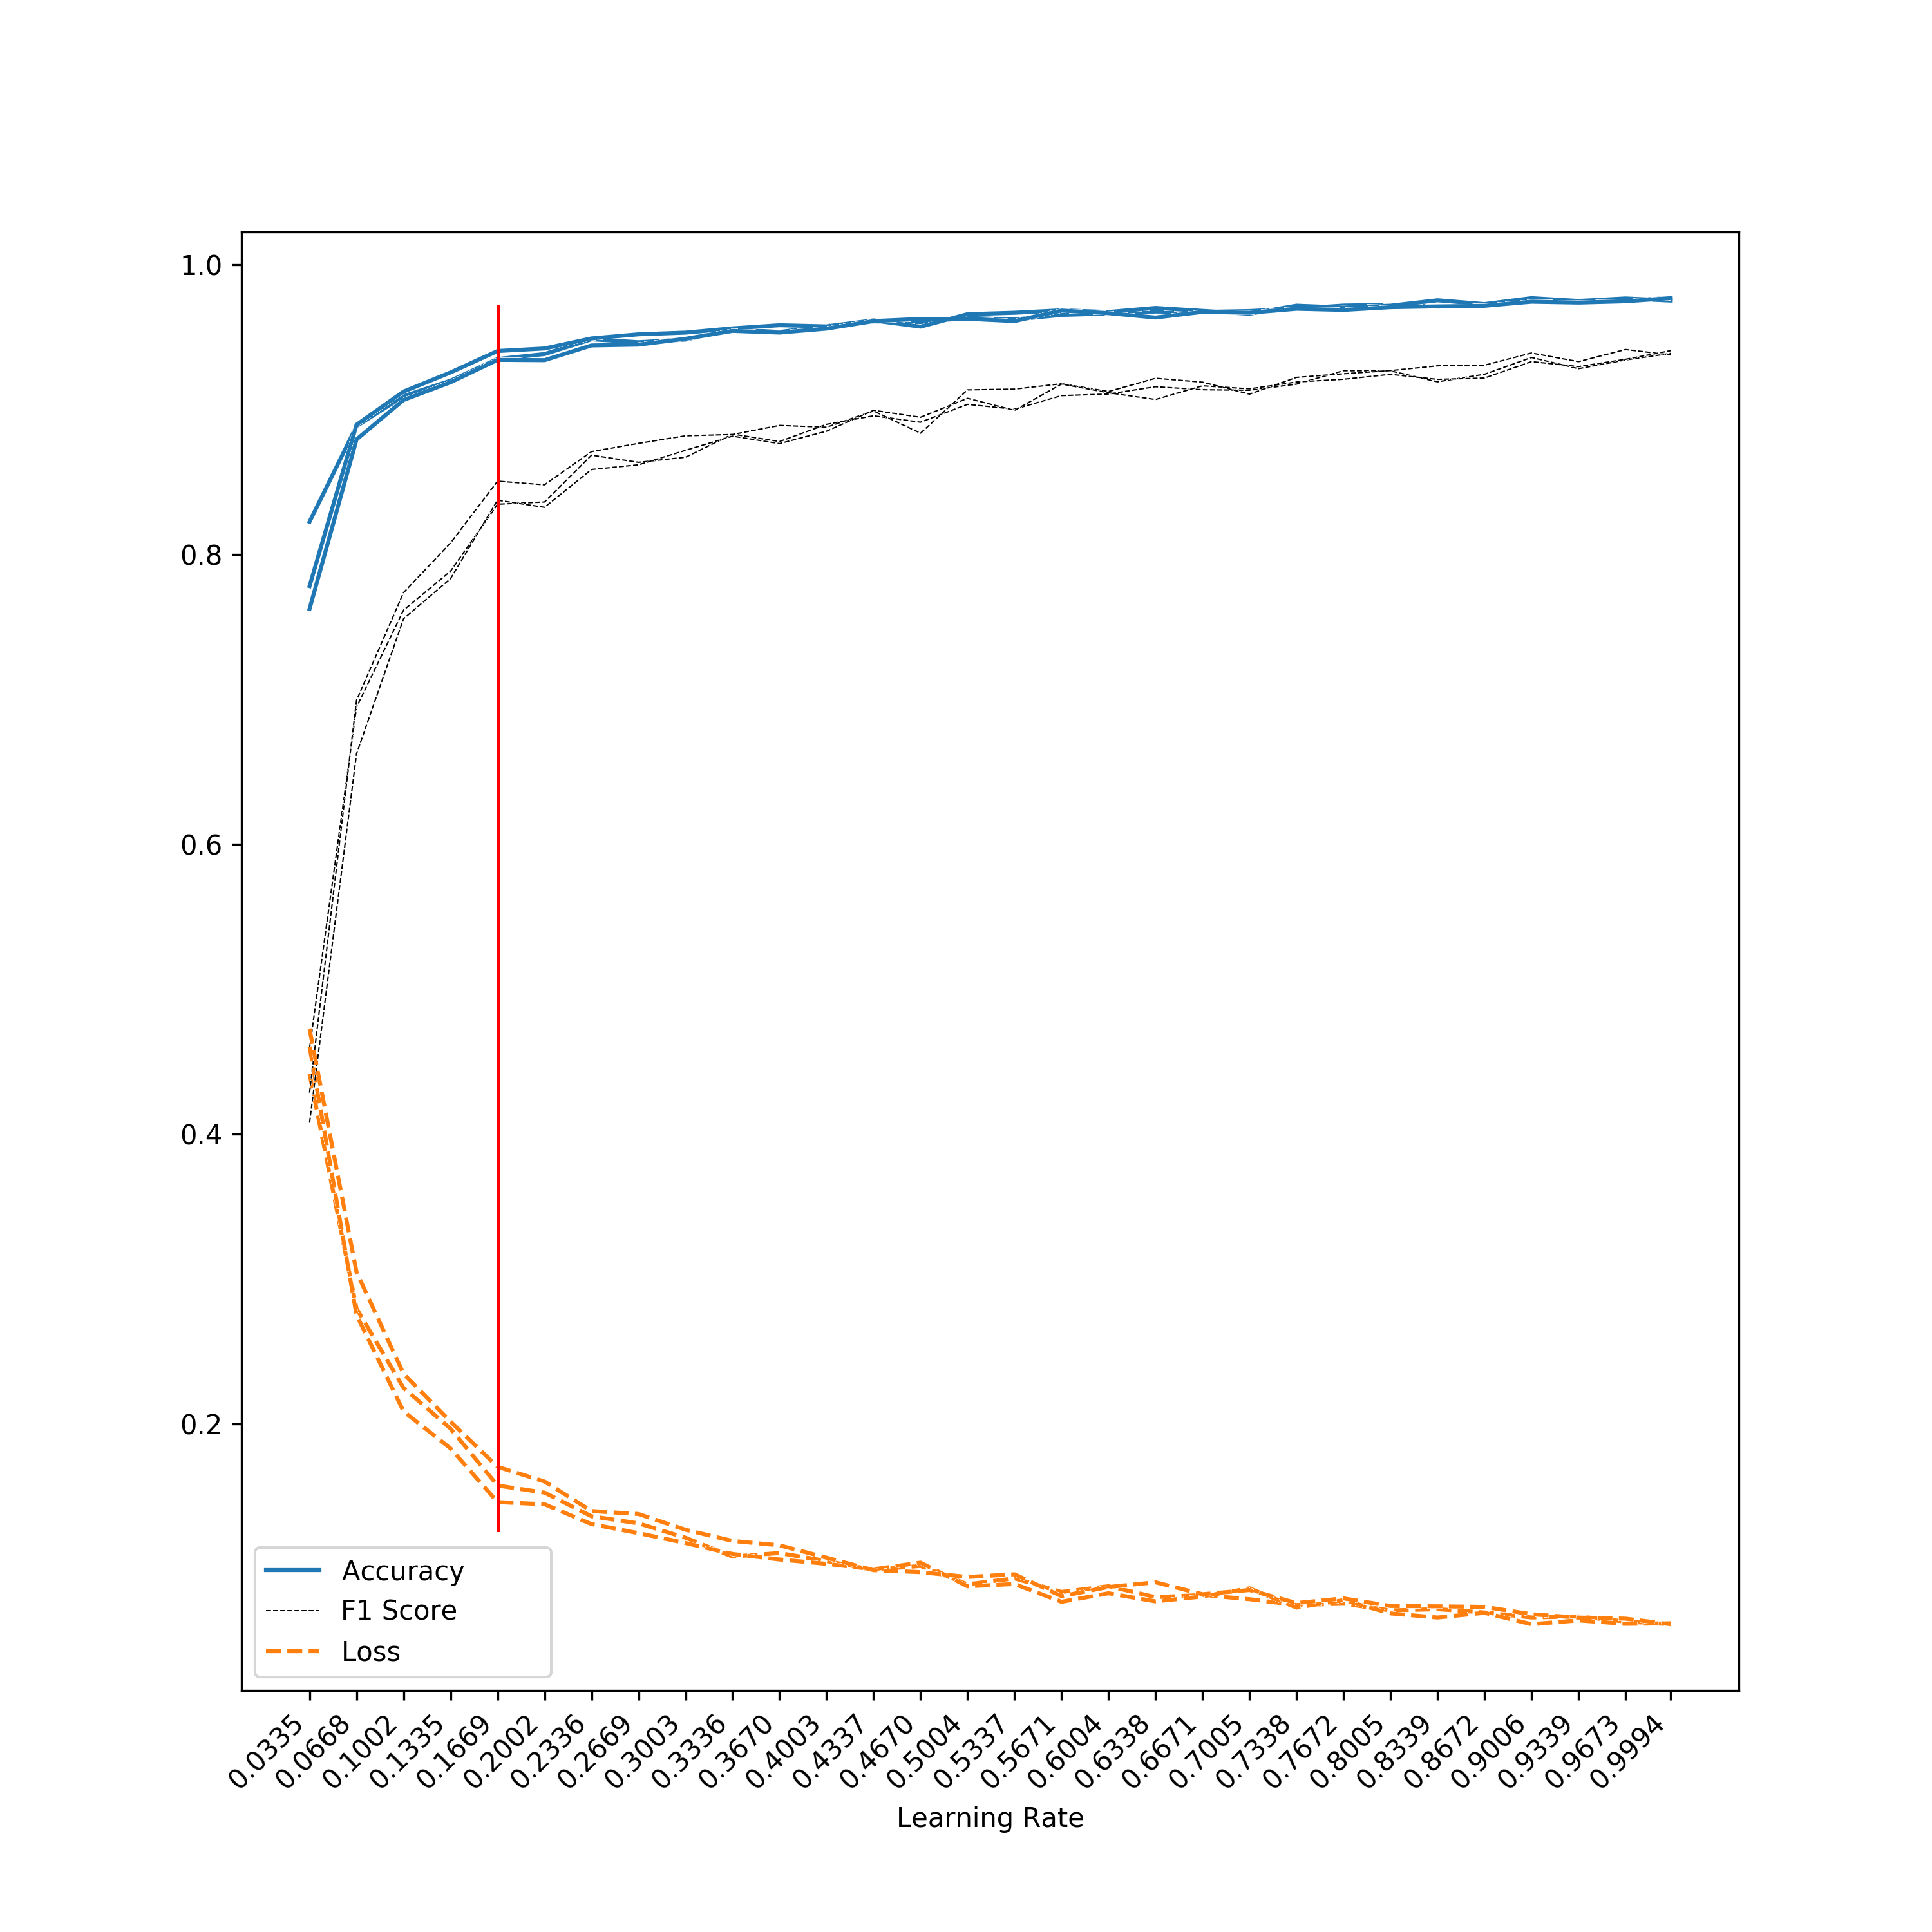
\includegraphics[height=0.45\textheight]{figures/appendix/lr_default}
    \caption{Lernraten Range Test für Default Konfiguration}
    \label{fig:apx:lr_default}
\end{figure}
\begin{figure}[H]
    \centering
    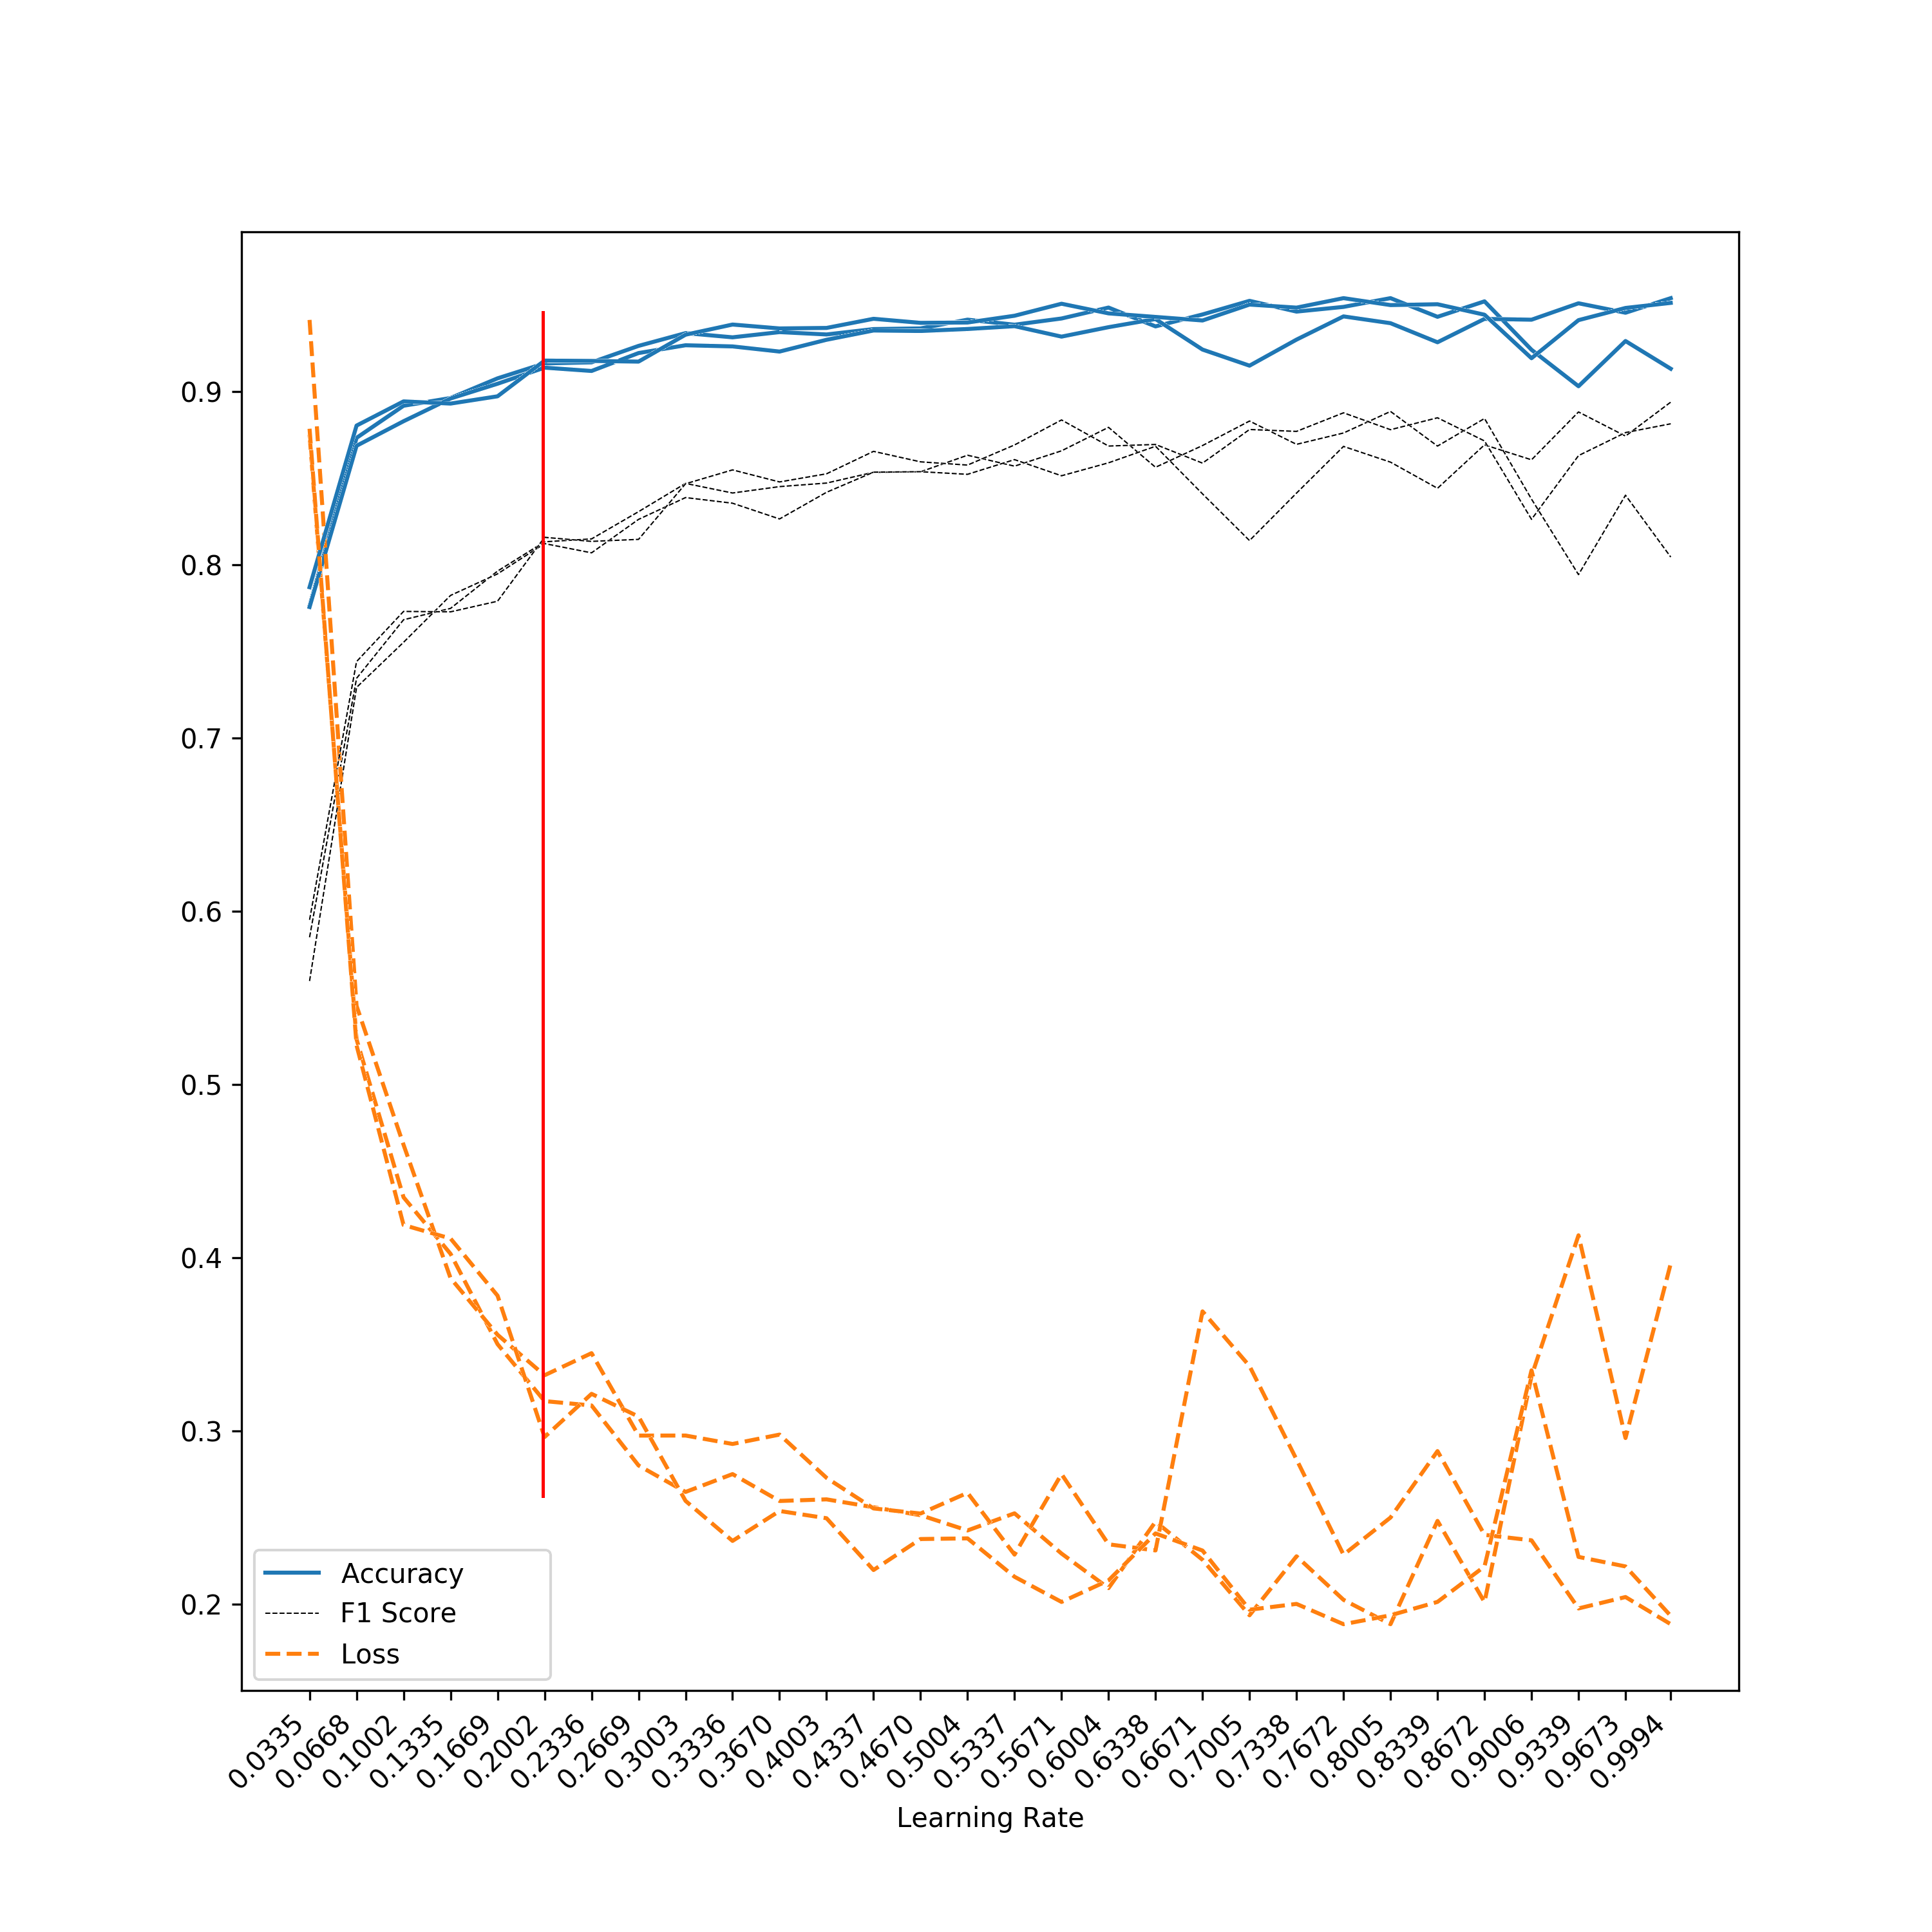
\includegraphics[height=0.45\textheight]{figures/appendix/lr_weighted}
    \caption{Lernraten Range Test für Gewichteter Loss Konfiguration}
    \label{fig:apx:lr_weighted}
\end{figure}
\begin{figure}[H]
    \centering
    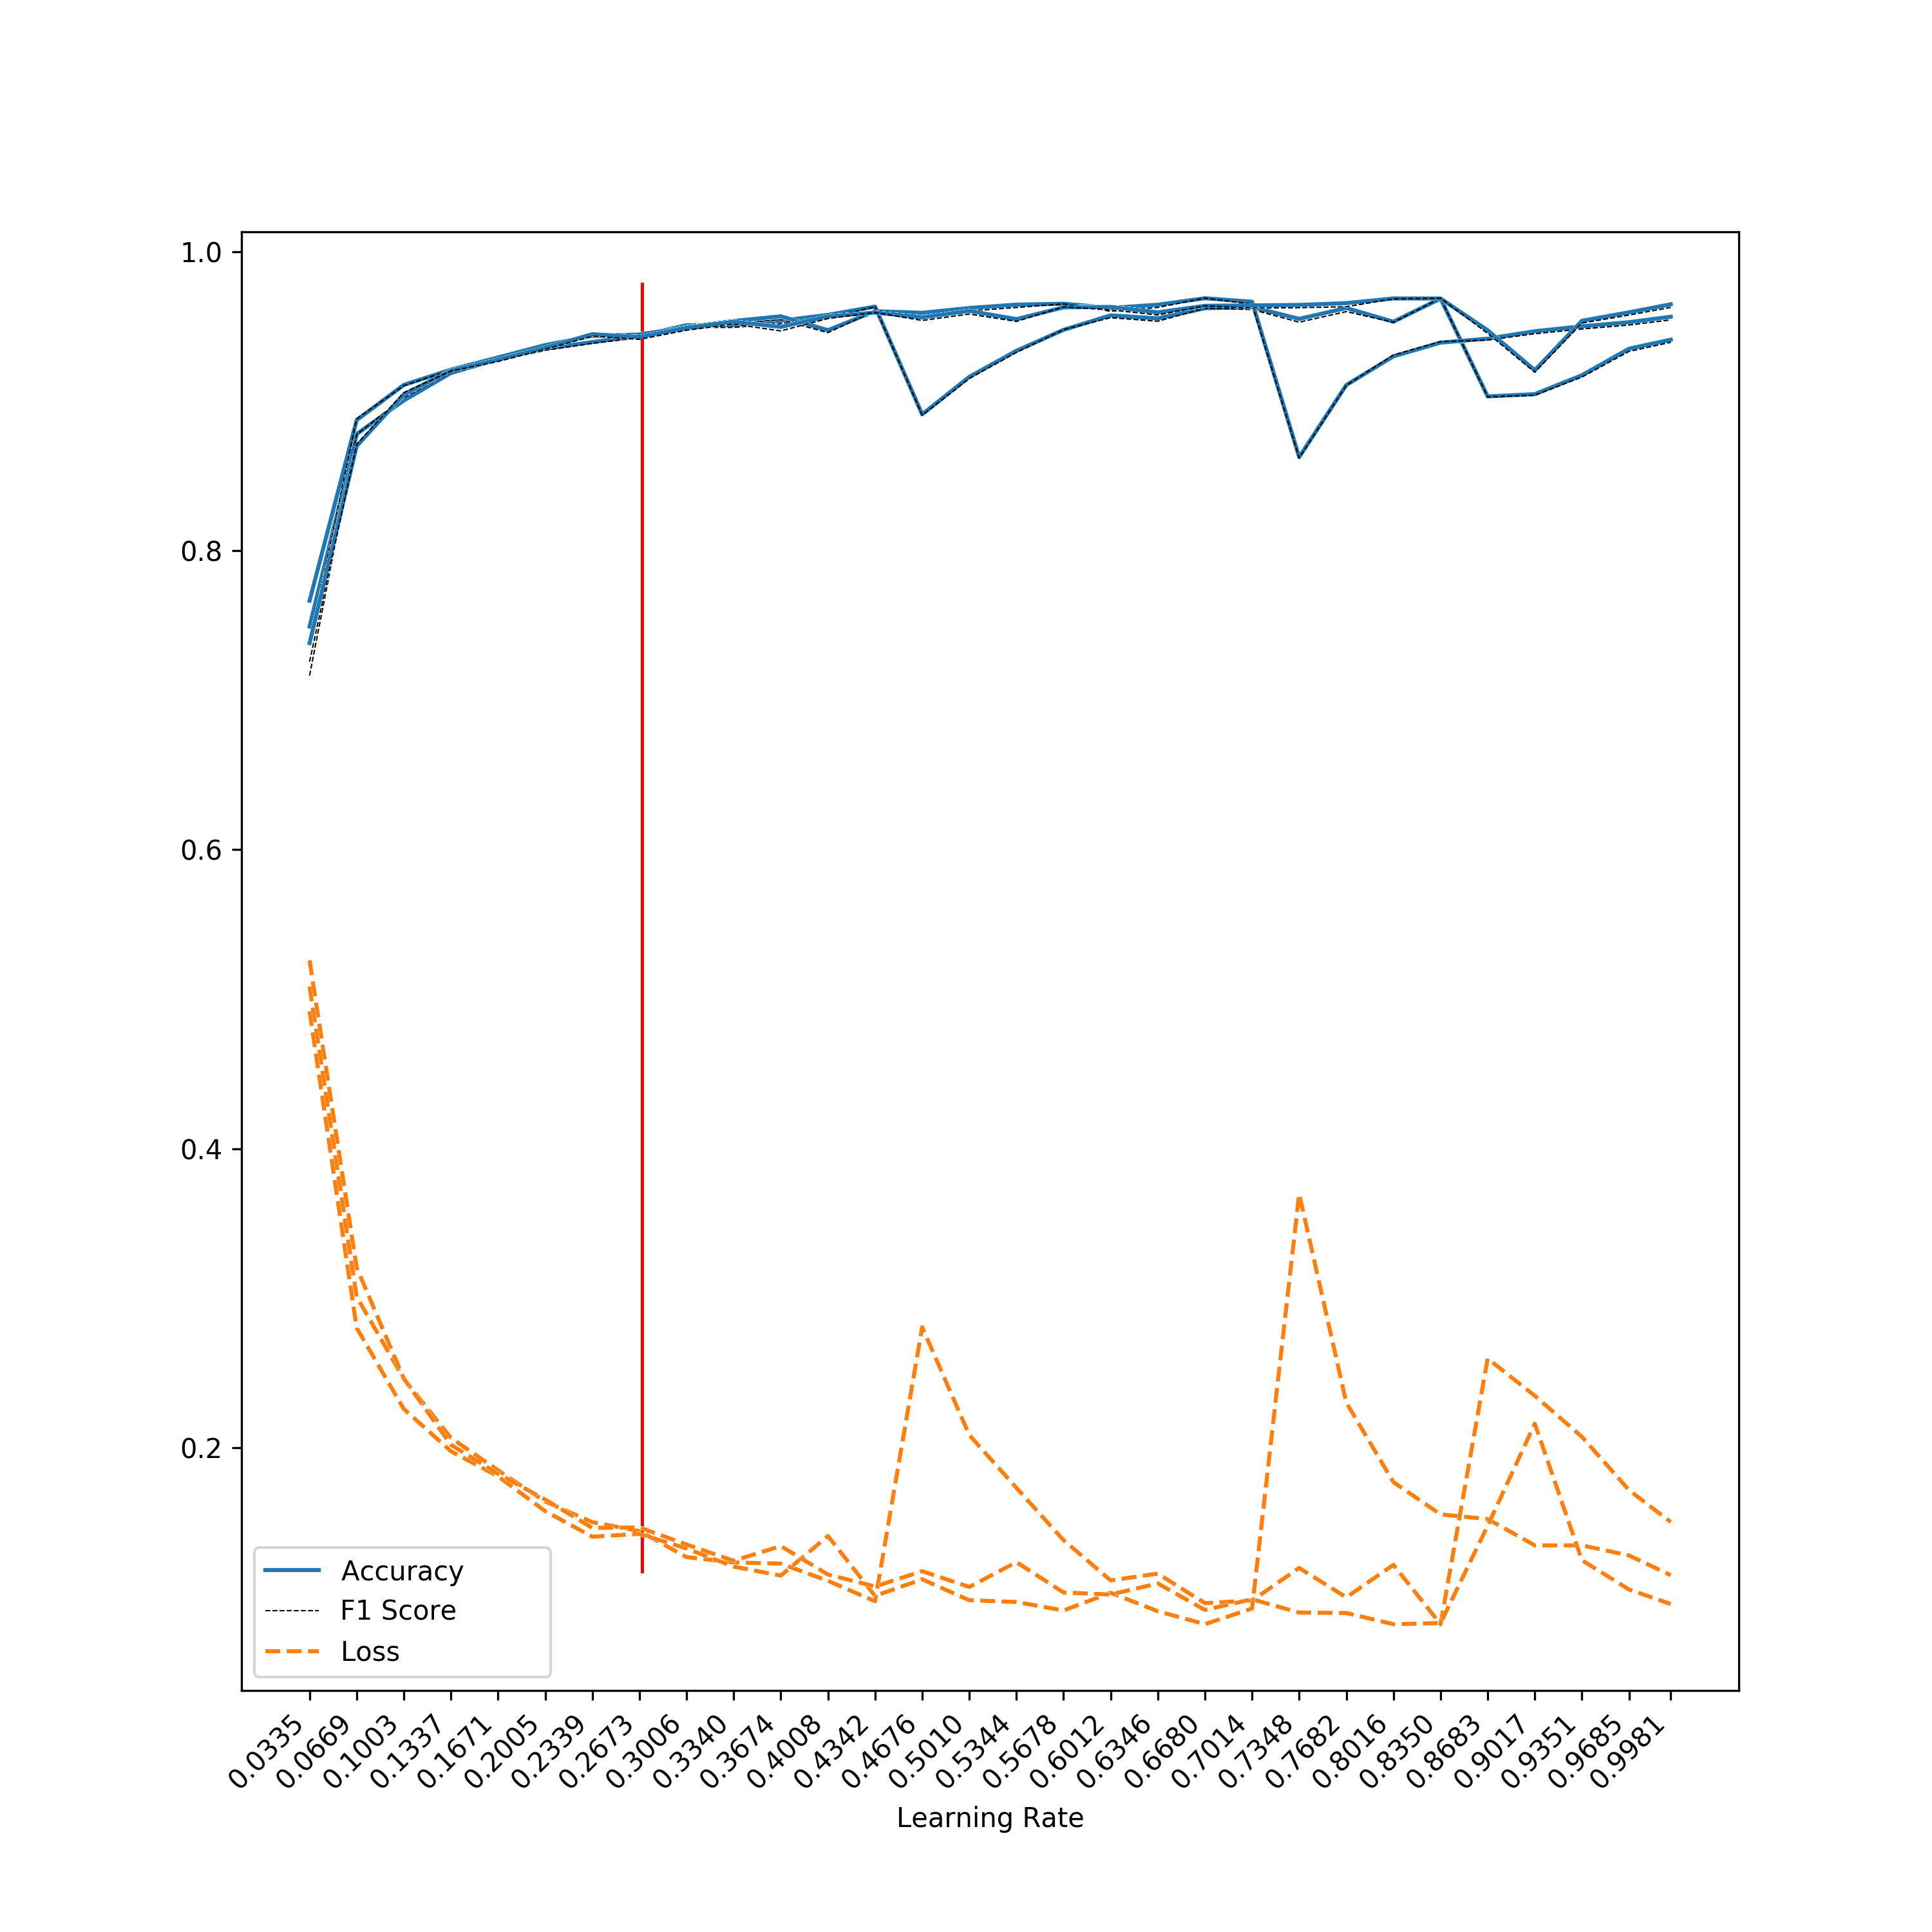
\includegraphics[height=0.45\textheight]{figures/appendix/lr_up}
    \caption{Lernraten Range Test für Hochgesampelte Konfiguration}
    \label{fig:apx:lr_up}
\end{figure}

\subsection*{EFN-N6 bis EFN-N15}
\begin{figure}[H]
    \centering
    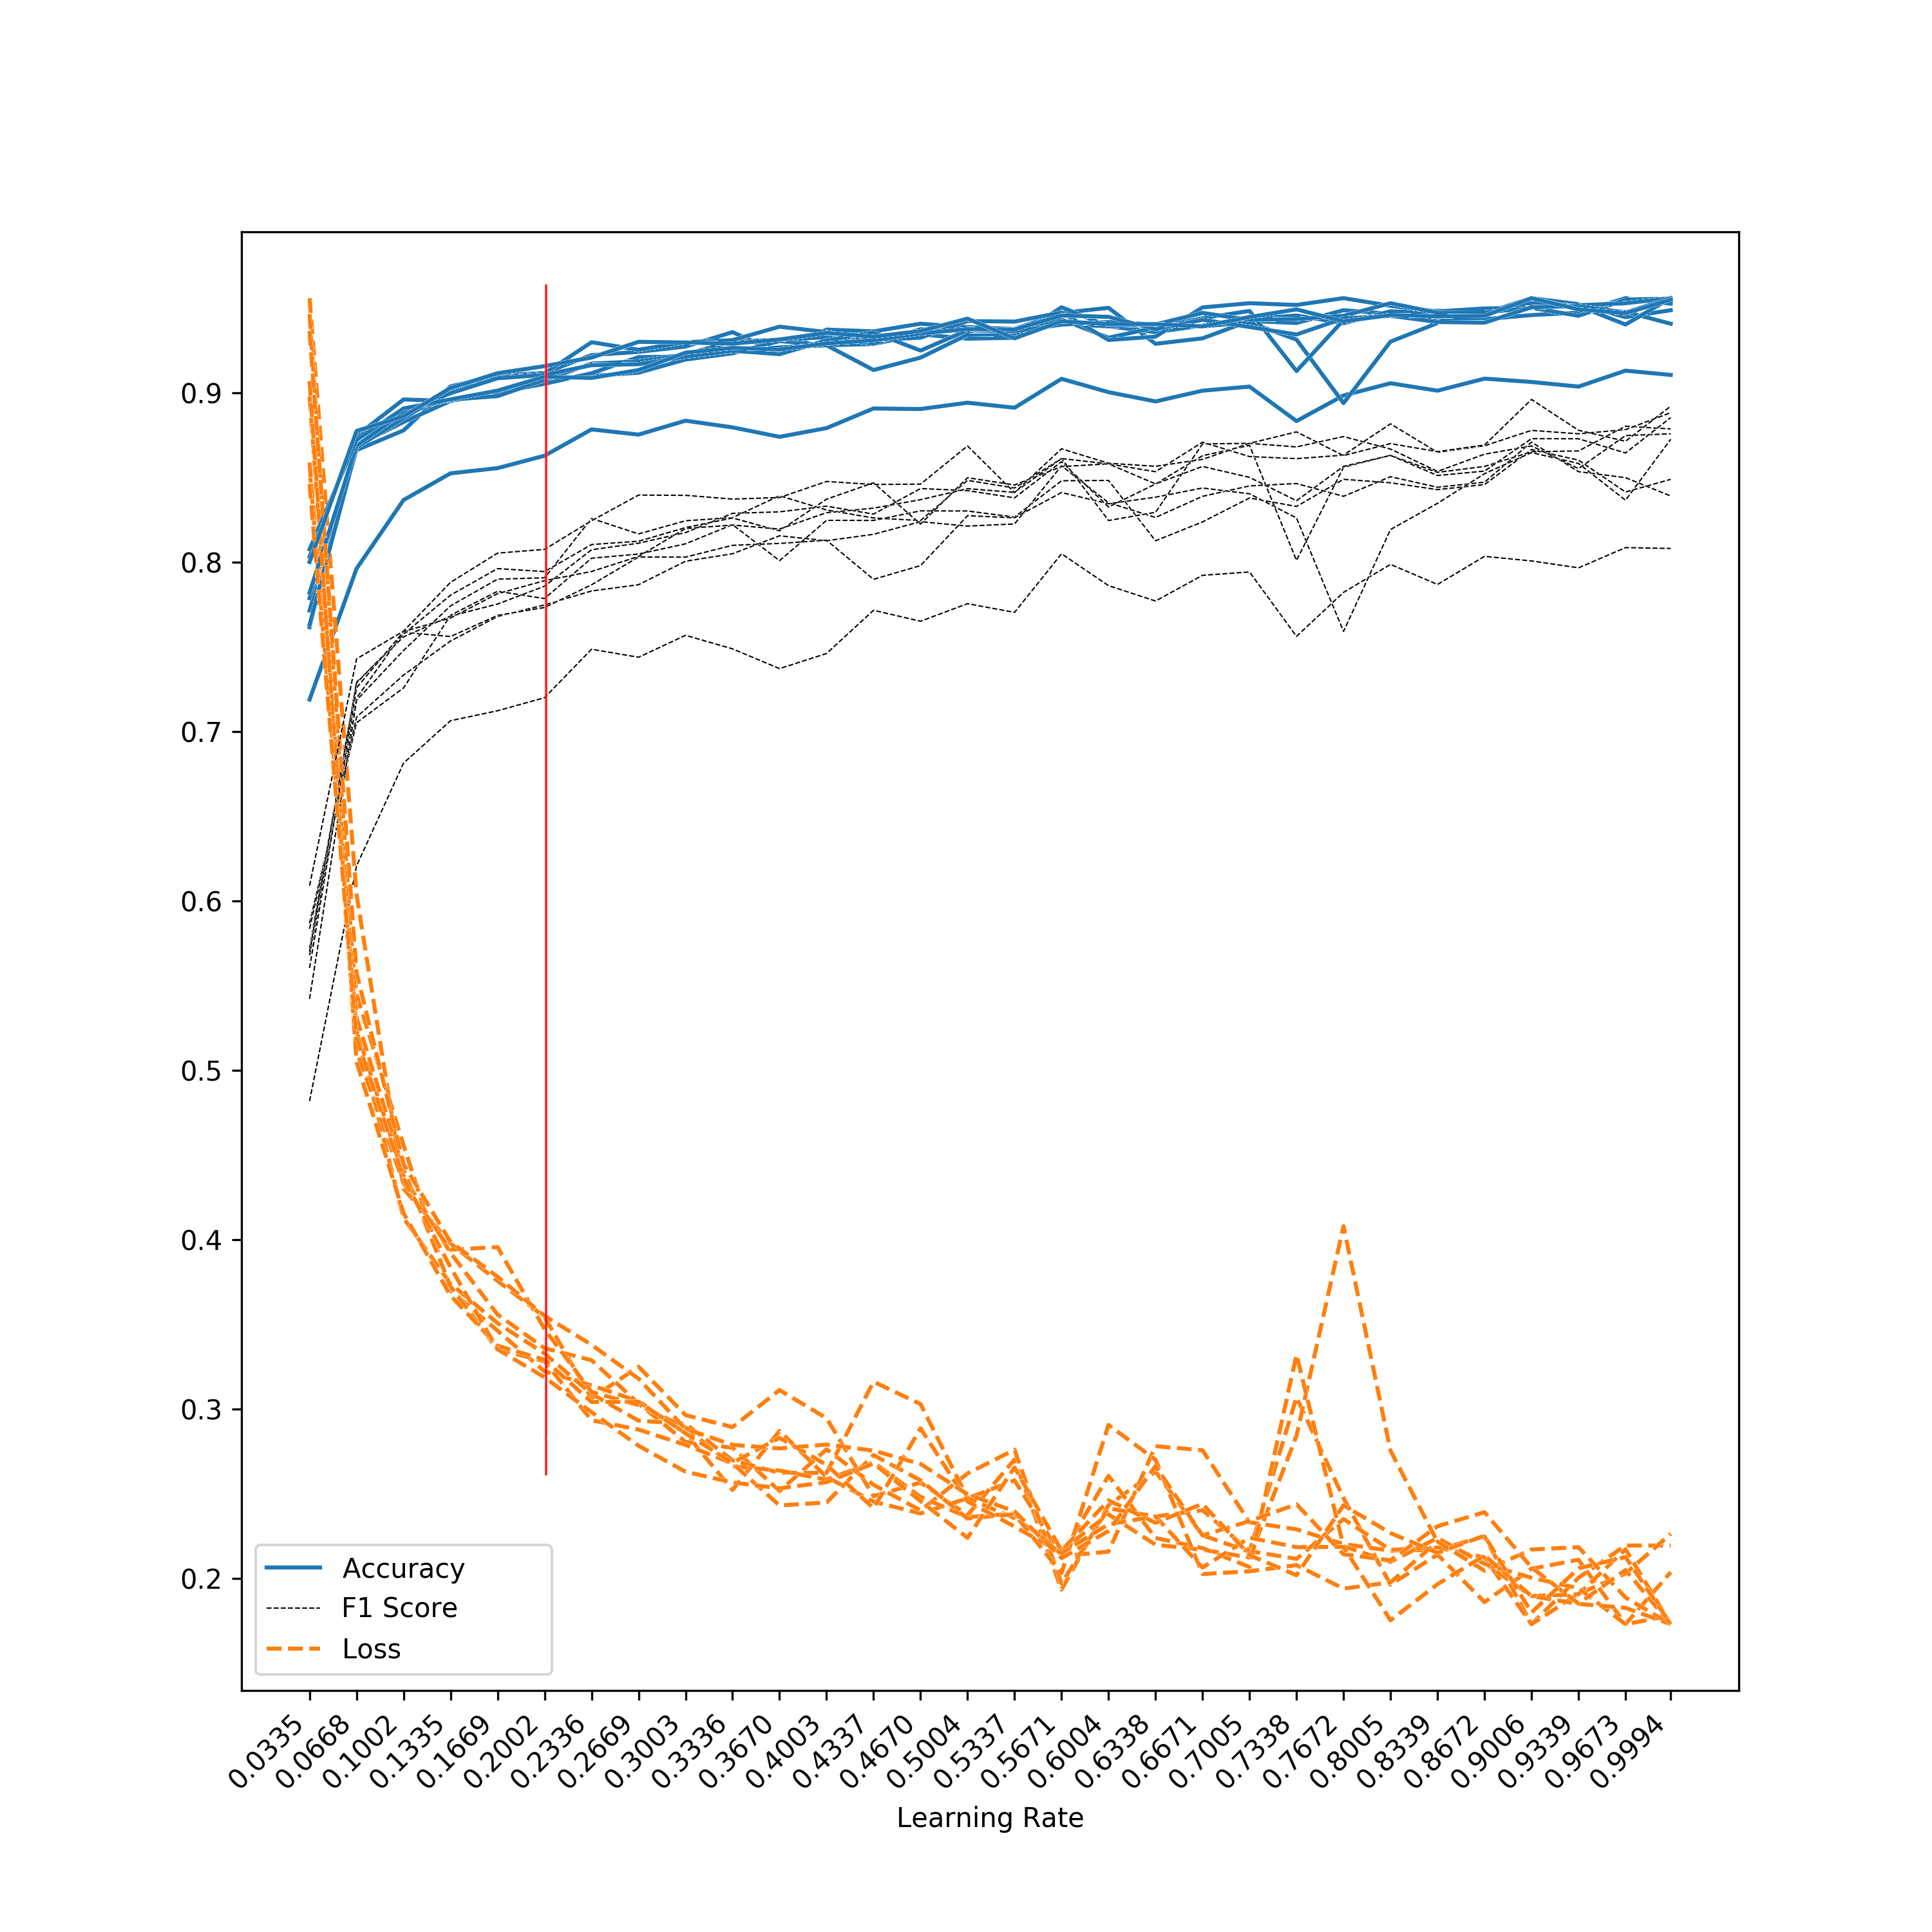
\includegraphics[height=0.45\textheight]{figures/appendix/lr_downscaled}
    \caption{Lernraten Range Test für EFN $\phi = [-6, -15]$}
    \label{fig:apx:lr_down}
\end{figure}

\section{Parameter für BMOG Skalierung} \label{apx:bmog_scale}
Die Postprocessinganzahl muss ungerade sein, da sie die Kernelgröße für den verwendeten \TT{MedianBlur} angibt.
Der wiederum benötigt einen Mittelpunkt, was nur bei ungeraden Größen möglich ist, da Pixel diskret sind.
Aus Einfachheitsgründen wurden für die Dilatation und Mindestgröße die gleichen Werte gewählt.

\begin{table}[ht]
    \centering
    \begin{tabular}{c|cc|cc}
    \BF{Skalierung} &
    \BF{$\text{Threshold}_L$} &
    \BF{Postprocessing} &
    \BF{Dilatation} &
    \BF{Mindestgröße} \\ \shline

    1.0 & 20 & 15 & 15 & 15 \\ \hline
    0.9 & 20 & 13 & 13 & 13 \\ \hline 
    0.8 & 20 & 13 & 13 & 13 \\ \hline 
    0.7 & 20 & 11 & 11 & 11 \\ \hline 
    0.6 & 20 & 9  & 9  & 9  \\ \hline 
    0.5 & 20 & 7  & 7  & 7  \\ \hline 
    0.4 & 20 & 7  & 7  & 7  \\ \hline 
    0.3 & 20 & 5  & 5  & 5  \\ \hline 
    0.2 & 20 & 5  & 5  & 5  \\ \hline 
    0.1 & 20 & 5  & 5  & 5  \\ \hline 
    \end{tabular}
    \caption{Parameter für die BMOG Skalierung}
    \label{apx:tab:bmog_scale}
\end{table}